\documentclass[a4paper,14pt]{report}
\usepackage[left=3cm,right=1cm,
    top=2cm,bottom=2cm,bindingoffset=0cm]{geometry}
\usepackage{amsmath,amsthm,amssymb}
\usepackage[T1,T2A]{fontenc}
\usepackage[utf8]{inputenc}
\usepackage[english,russian]{babel}
\usepackage{graphicx}
\usepackage{wrapfig}
\graphicspath{{pictures/}}
\DeclareGraphicsExtensions{.pdf,.png,.jpg,.gif}


%\date{}

\begin{document}

\tableofcontents{}
%\clearpage

\chapter{Основы криптографии}
\section{История появления необходимости криптографии}

Человечеству всегда было необходимо передавать информацию так, чтобы её могли получить лишь те, кому она назначена, и не попала в руки к тем, от кого её берегли. С изобретением письменности это стало намного актуальнее, и именно тогда появилось понятие тайнописи. Люди пробовали самые различные методы утаивания информации- от использования особых чернил, которые либо через время исчезали с бумаги, либо которые были видны только при контакте с особыми химическими реагентами, до скрытия основной информации в большом тексте.
Криптография появилась именно как наука, изучающая способы шифрования данных, а именно обезопасить данные не сокрытием факта их передачи, а сделав содержимое недоступным посторонним, даже если они завладеют ими(данными). Для этого информацию нужно исказить таким образом, чтобы содержимое было понятно только корреспондентам, и никому более.
В 1950-х, с появлением первых \textbf{ЭВМ} ситуация значительно изменилась- криптография обрела полноценный практический смысл, уйдя от понятия \textbf{“тайнопись”}. На сегодняшний день эта дисциплина включает в себя методы защиты информации и информационных взаимодействий различного характера, основываясь на преобразовании данных секретными алгоритмами, а также на алгоритмах, включающих в себя секретные параметры. Информационным взаимодействием называется процесс обмена, передачи и обработки информации между двумя и более субъектами. Основных, фундаментальных методов преобразования в современной криптографии не столь много, но комбинируя их можно получить полноценную прикладную систему.
Информация является самым важным ресурсом современной жизни. Компьютерные сети и Интернет упростили доступ к данным о конкретных людях, так и о финансовых и государственных организациях. Очевидно, что этим могут воспользоваться злоумышленники. Как говорилось ранее, криптография является совокупностью способов преобразования (т.е. шифрования)  информации, сделав её бесполезной в случае попадания данных в руки неправомерных пользователей.
Сегодня, криптография и её методы применяются для идентификации пользователей и их аутентификации,  защиты каналов связи и передачи данных, защита электронных документов от изменения и копирования.

\section{Основные понятия криптографии и их реализации}
\textbf{Основной механизм защиты данных} — это \textbf{шифрование}.    
\textbf{Шифрование —} это преобразование информации в нечитабельную форму, осуществляемое с помощью ключей шифрования. Методов шифрования имеется множество, среди которых есть элементарные, так и принципиально невозможные для вскрытия. Ниже представлена обобщенная схема криптосистемы, обеспечивающей шифрование данных.

\begin{figure}[h]
\center{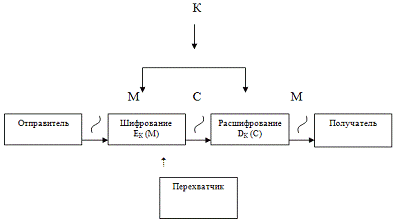
\includegraphics[scale=0.5]{image1.png}}
\caption{Обобщенная схема криптосистемы}
\label{fig:image}
\end{figure}

Отправитель составляет понятный текст первоначального сообщения M, которое будет передано по незащищённому каналу Получателю. Чтобы Перехватчик не смог воспользоваться содержимым сообщения даже после перехвата, сообщение М шифруется при помощи обратимого преобразования $Е_{к}$ и получается криптограмма $С = E_{к}(M)$. Получатель, приняв криптограмму, расшифровывает её при помощи  обратного преобразования $D = E{_k}^{-1}$ и получает открытое содержимое сообщения
\hfill \break
 $M: D_k(C) = E{_k}^{-1}(E_k(M)) = M.$
\hfill \break
Все преобразования выбираются из так называемого семейства криптографических преобразований, называемых \textbf{криптоалгоритмами.} Параметр, по которому выбирается конкретное криптографическое преобразование, называется криптографическим ключом $К$. Ключ $К$ принадлежит определенному пользователю или группе пользователей и быть для них уникальным. Информация, зашифрованная с использованием определённого ключа может быть расшифрована лишь владельцем или владельцами ключа.
\hfill \break
Говоря в целом, шифрование бывает симметричным или асимметричным в отношении преобразования расшифрования. 
\hfill \break
\textbf{Это свойство разделяет практически все криптосистемы на две части:}

\begin{itemize}
  \item Симметричные криптосистемы (один ключ)
  \item Асимметричны криптосистемы (два ключа)
  \end{itemize}

В случае с симметричной криптосистемой используются идентичные ключи в блоке шифрования и в блоке расшифрования. То есть, владея ключом шифрования, можно беспрепятственно расшифровать сообщение. Из-за этого симметричные криптосистемы так же называют криптосистемами с секретным ключом- потому что ключ шифрования должен быть доступен лишь тем, кому дозволена информация в сообщении. Следовательно, задача сохранения конфиденциальности сообщений и/или электронных документов сводится к сохранению конфиденциальности этого самого ключа шифрования.
Одно из основных неудобств симметричного шифрования заключается в том, что перед обменом зашифрованными данными надо обменяться секретными ключами между адресатами. Нельзя допускать, чтобы этот обмен происходил в общедоступных каналах связях, ключ должен быть передан по защищённому специальному каналу распространения ключей.
Симметричное шифрование хорошо подходит для шифрования с целью защитить архивные файлы, а также для шифрования логических и физических дисков.
Принципиальное отличие ассиметричной системы шифрования от симметричной заключается в том, что для расшифрования используется ключ, отличающийся от ключа для шифрования. В таком случае, первый ключ является открытым, а второй- секретным.

Криптоанализ- наука о раскрытии первоначального текста зашифрованного сообщения без ключа. Успех такого анализа может раскрыть не только исходный текст, но и ключ. Также, можно выяснить слабые места криптосистемы и позже исправить их.
Основополагающим правилом этой науки сформулировал голландец \textbf{А. Керхоффом}, заключив, что стойкость шифра должна определяться только секретностью ключа. Иначе говоря, это правило указывает на то, что весь алгоритм, кроме значения секретного ключа, известен \textbf{крипто-аналитику.} Это обусловлено тем, что любая криптосистема, реализующая семейство преобразований, рассматривается как открытая. 

\chapter{Хэширование}
\section{Разновидности хэширования}
Как было упомянуто выше, криптография занимается не только конфиденциальностью данных, но и её целостностью. Контроль этой самой целостности осуществляется, в основном, с помощью расчета \textbf{“контрольной суммы”} данных. Для большинства приложений достаточно простой контрольной суммы, однако чтобы сделать криптографически стойкие контрольные суммы, необходимо использование хэш-функций.

Базовыми свойствами криптографически стойкой хэш-функции являются свойства рассеивания и стойкости к коллизиям.
Коллизией хэш-функции H называется случай, в котором существуют два различных текста Т1 и Т2, но H(T1)=H(T2). Значение хэш-функции имеет фиксированную длину, а длина текста не ограничена. Следовательно, коллизии существуют. Стойкость к коллизиям означает то, что для текста Т1 невозможно найти текст Т2, вызывающий коллизию.
Свойство рассеивания означает, что минимальное изменение текста будет вызывать максимальные изменения в значении хэш-функции.
Основными алгоритмами хэш-функций, применяемым на сегодняшний день, являются \textbf{MD2, MD4, MD5, SHA} (а также его разновидность, SHA1). Типичные длины хэш-функций разнятся от 16 до 32 байт.
Здесь стоит отметить важный аспект современного цифрового мира, объединяющий асимметричное шифрование и хэш-функции- электронная подпись. Электронная подпись документа- хэш сумма, зашифрованная секретным ключом. Если зашифровать сообщение секретным ключом, парным к открытому, то любой желающий сможет расшифровать содержимое. Проверка электронной подписи заключается в вычислению хэш-суммы документа, в вычислений хэш-суммы подписи и сравнения данных величин. Если значения равны, то подпись под документом считается верной.
\section{SHA-1}
\textbf{Secure Hash Algorithm 1 —} алгоритм криптографического хэширования. Входное сообщение генерируется в 160-битное хеш-значение. SHA-1 реализует хэш-функцию, основывающуюся на функции сжатия. Входами функции сжатия являются блок текста длиной 512 бит выход предыдущего блока сообщения. Выход является значением хэш-блоков до этого момента, то есть хэш блока $M_i$ равен $H=f(M_i H_{i-1})$. Хэш значением всего сообщения является последний блох выхода. Хэш значением всего сообщения является последний блох выхода.

\subsection{Коллизии SHA-1}

В официальном сообщении авторы говорят, что эта находка стала результатом двухлетнего исследования, которая началась вскоре после публикации в 2013 году работы криптографа Марка Стивенса из Центра математики и информатики в Амстердаме о теоретическом подходе к созданию коллизии SHA-1. Он же в дальнейшем продолжил поиск практических методов взлома вместе с коллегами из Google.

Компания Google давно выразила своё недоверие SHA-1, особенно в качестве использования этой функции для подписи сертификатов TLS. Ещё в 2014 году, вскоре после публикации работы Стивенса, группа разработчиков Chrome объявила о постепенном отказе от использования SHA-1. Теперь они надеются, что практическая атака на SHA-1 увеличит понимание у сообщества информационной безопасности, так что многие ускорят отказ от SHA-1.

Чтобы представить число хешей, которые обсчитала Google во время брутфорса, можно упомянуть, что примерно такое же количество хешей SHA-256 обсчитывается в сети Bitcoin каждые три секунды, так что в атаке нет ничего фантастического. Вполне можно предположить, что в криптографических отделах некоторых организаций с большими дата-центрами уже давно обсчитываются коллизии SHA-1.

Сейчас Марк Стивенс с соавторами опубликовали научную работу, в которой описывают общие принципы генерации документов с блоками сообщений, которые подвержены коллизии SHA-1.

\begin{figure}[h]
\center{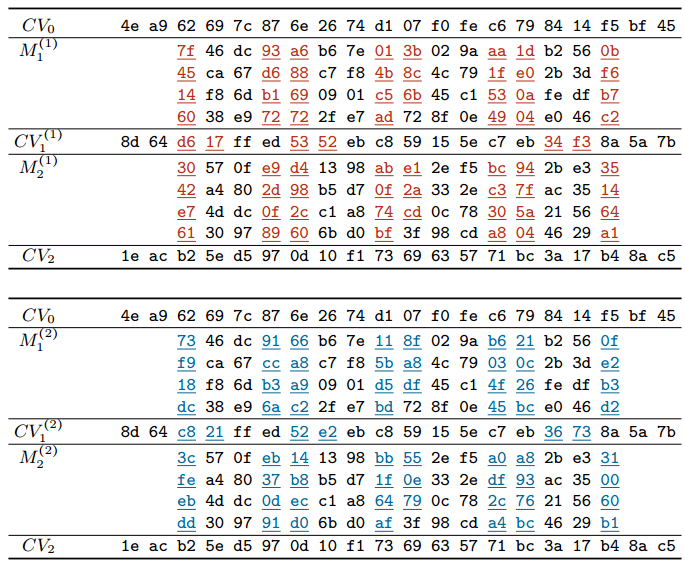
\includegraphics[scale=0.4]{image7.png}}
\label{fig:image}
\end{figure}




\section{MD5}
\textbf{MD5 (англ. Message Digest 5) —} 128-битный алгоритм хеширования, разработанный профессором Рональдом Л. Ривестом из Массачусетского технологического института (Massachusetts Institute of Technology, MIT) в 1991 году. Предназначен для создания \textbf{«отпечатков»} или \textbf{дайджестов сообщения произвольной длины и последующей проверки их подлинности.} Широко применялся для проверки целостности информации и хранения хешей паролей.

На вход алгоритма поступает входной поток данных, хеш которого необходимо найти. Длина сообщения измеряется в битах и может быть любой (в том числе нулевой). Запишем длину сообщения в L. Это число целое и неотрицательное. Кратность каким-либо числам необязательна. После поступления данных идёт процесс подготовки потока к вычислениям.

\hfill \break

 В данном алгоритме предполагается наличие 5 шагов, а именно:
\begin{enumerate}
  \item Выравнивание потока
  \item Добавление длины сообщения
  \item Инициализация буфера
  \item Вычисление в цикле
  \item Результат вычислений
 \end{enumerate}
 
 \textbf{На первом шаге} \textit{“Выравнивание потока”} сначала дописывают единичный бит в конец потока, затем необходимое число нулевых бит. Входные данные выравниваются так, чтобы их новый размер был сравним с 448 по модулю 512. Выравнивание происходит, даже если длина уже сравнима с 448.
 
 \textbf{На втором шаге} в оставшиеся 64 бита дописывают 64-битное представление длины данных до выравнивания. Сначала записывают младшие 4 байта. Если длина превосходит $2^{64}-1$, то дописывают только младшие биты. После этого длина потока станет кратной 512. Вычисления будут основываться на представлении этого потока данных в виде массива слов по 512 бит.
 
\textbf{На третьем} для вычислений используются четыре переменные размером 32 бита и задаются начальные значения в 16-ричном виде. В этих переменных будут храниться результаты промежуточных вычислений.

\textbf{Во время 4-го шага} \textit{“Вычисление в цикле”} происходит 4 раунда, в которых сохраняются значения, оставшиеся после операций над предыдущими блоками. После всех операций суммируются результаты двух последних циклов. Раундов в MD5 стало 4 вместо 3 в MD4. Добавилась новая константа для того, чтобы свести к минимуму влияние входного сообщения. В каждом раунде на каждом шаге и каждый раз константа разная. Она суммируется с результатом и блоком данных. Результат каждого шага складывается с результатом предыдущего шага. Из-за этого происходит более быстрое изменение результата. Изменился порядок работы с входными словами в раундах \textbf{2 и 3.}

\textbf{В итоге на 5-ом шаге} мы получим результат вычислений, который находится в буфере -это и есть хеш. Если выводить побайтово, начиная с младшего байта первой переменной и закончив старшим байтом последней, то мы получим MD5-хеш. 

\subsection{Уязвимости MD5}
Алгоритм MD5 уязвим к некоторым атакам. Например, возможно создание двух сообщений с одинаковой хеш-суммой.

На данный момент существуют несколько видов взлома хешей \textbf{MD5 — подбора сообщения с заданным хешем:}
\begin{itemize}
  \item Перебор по словарю
  \item Brute-force
  \item RainbowCrack
  \item Коллизия хеш-функции
  \end{itemize}

При этом методы перебора по словарю и \textbf{brute-force} могут использоваться для взлома хеша других хеш-функций (с небольшими изменениями алгоритма). \textbf{RainbowCrack} требует предварительной подготовки радужных таблиц, которые создаются для заранее определённой хеш-функции. Поиск коллизий специфичен для каждого алгоритма. Рассмотрим каждый вид \textbf{«взлома»} по отдельности.

\subsection{Атаки переборного типа}
В криптографии атака полного перебора или исчерпывающий поиск ключей -это стратегия, которая теоретически может быть использована против любых зашифрованных данных. Злоумышленник, который не может воспользоваться слабостью в системе шифрования, реализовывает атаку подобного типа. Она включает в себя систематическую проверку всех возможных ключей, пока не будет найден правильный. В худшем случае для взлома сообщения потребуется задействовать всю вычислительную мощность. 
Перебор по словарю — атака на систему защиты, применяющая метод полного перебора предполагаемых паролей, используемых для аутентификации, осуществляемого путём последовательного пересмотра всех слов (паролей в чистом виде) определённого вида и длины из словаря с целью последующего взлома системы и получения доступа к секретной информации.
Как видно из определения, атаки по словарю являются атаками полного перебора. Единственное отличие состоит в том, что данные атаки обычно более эффективны так как становится не нужным перебирать все комбинации символов, чтобы добиться успеха. Злоумышленники используют обширные списки наиболее часто используемых паролей таких как, имена домашних животных, вымышленных персонажей или конкретно характерных слов из словаря – отсюда и название атаки. Однако если пароль действительно уникален (не является комбинацией слов), атака по словарю не сработает. В этом случае использование атаки полного перебора -единственный вариант.
Для полного перебора или перебора по словарю можно использовать программы \textbf{PasswordsPro}, \textbf{MD5BFCPF}, \textbf{John the Ripper.} Для перебора по словарю существуют готовые словари.

\subsection{RainbowCrack}
Это ещё один метод взлома хеша. Он основан на генерировании большого количества хешей из набора символов, чтобы по получившейся базе вести поиск заданного хеша.
Радужные таблицы состоят из хеш-цепочек и более эффективны, чем предыдущий упомянутый тип атак, поскольку они оптимизируют требования к хранению, хотя поиск выполняется немного медленнее. Радужные таблицы отличаются от хеш-таблиц тем, что они создаются с использованием как хеш-функций, так и функций редукции.
\textbf{Цепочки хешей —} метод для уменьшения требования к объёму памяти. Главная идея — определение функции редукции R, которая сопоставляет значениям хеша значения из таблицы. Стоит отметить, что R не является обращением хеш-функции.
Радужные таблицы являются развитием идеи таблицы хеш-цепочек. Функции редукции применяются по очереди, перемежаясь с функцией хеширования.
Использование последовательностей функций редукции изменяет способ поиска по таблице. Поскольку хеш может быть найден в любом месте цепочки, необходимо сгенерировать несколько различных цепочек.
Существует множество систем взлома паролей и веб-сайтов, которые используют подобные таблицы. Основная идея данного метода — достижение компромисса между временем поиска по таблице и занимаемой памятью. Конечно, использование радужных таблиц не гарантирует 100\% успеха взлома систем паролей. Но чем больше набор символов, используемый для создания радужной таблицы, и чем продолжительнее хеш-цепочки, тем больше будет шансов получить доступ к базе данных исходных паролей.

\subsection{Коллизии MD5}
\textbf{Коллизия хеш-функции —} это получение одинакового значения функции для разных сообщений и идентичного начального буфера. В отличие от коллизий, псевдоколлизии определяются как равные значения хеша для разных значений начального буфера, причём сами сообщения могут совпадать или отличаться. В 1996 году Ганс Доббертин нашёл псевдоколлизии в MD5, используя определённые инициализирующие векторы, отличные от стандартных. Оказалось, что можно для известного сообщения построить второе такое, что оно будет иметь такой же хеш, как и исходное. С точки зрения математики, это означает следующее:
$MD5(I_V, L_1) = MD5(I_V, L_2),$
где $I_V$ — \textbf{начальное значение буфера}, а $L_1$ и $L_2$ — \textbf{различные сообщения.}
MD5 был тщательно изучен криптографическим сообществом с момента его первоначального выпуска и до 2004 года демонстрировал лишь незначительные недостатки. Однако летом 2004 года криптографы Ван Сяоюнь и Фэн Дэнго продемонстрировали алгоритм способный генерировать MD5-коллизии с использованием стандартного вектора инициализации.
Позже данный алгоритм был усовершенствован, как следствие время поиска пары сообщений значительно уменьшилось, что позволило находить коллизии с приемлемой вычислительной сложностью. Как оказалось, в MD5 вопрос коллизий не решается.


\chapter{Отечественные алгоритмы хэширования}
\section{Стрибог}
\textbf{Стрибог —} это семейство хеш-функций, включающее в себя всего две функции. Функцию с длиной выходного значения в 256 бит и функцию с длиной выходного значения в 512 бит. Обе эти функции имеют одинаковую структуру и отличаются друг от друга только начальным внутренним состоянием. Входными данными для обеих функций является блок данных длиной 512 бит. В случае, если длина сообщения больше 512 бит, то происходит разбиение сообщения на блоки. В случае же, если длина меньше 512 бит, то производится дополнение сообщения.

Прежде чем приступать к описанию алгоритма, расскажем о преобразованиях, которые используются при вычислении хеш-функции.
\subsection{Преобразования}

\begin{enumerate}
  \item \textbf{X-преобразование.} На вход функции X подаются две последовательности длиной 512 бит каждая, выходом функции является XOR этих последовательностей.
  
  $X[K] : V_{512} \rightarrow V_{512},     X[k](a) = k \oplus a, k, a \in V_{512}$
  
  \item \textbf{S - преобразование.} Функция \textbf{S} является обычной функцией подстановки. Каждый байт из 512-битной входной последовательности заменяется соответствующим байтом из таблицы подстановок $\pi$
  
   $S : V_{512} \rightarrow V_{512},    S(a) = S(a_{63}||...||a_0) = \pi(a_{63}||...||\pi(a_0)$
   
   Таблица $\pi$ является константой и может быть записана в виде массива
   
   \item \textbf{P-преобразование.} Функция перестановки. Для каждой пары байт из входной последовательности происходит замена одного байта другим. 
   
    $P : V_{512} \rightarrow V_{512},    P(a) = S(a_{63}||...||a_0) = a_{\tau(63)}||...||a_{\tau(0)}$
    
    Таблица перестановок $\tau$ также является константой
    
    \item \textbf{L-преобразование.} Представляет собой умножение 64-битного входного вектора на бинарную матрицу \textbf{A} размерами 64x64.
    
        $L : V_{512} \rightarrow V_{512},    L(a) = S(a_{7}||...||a_0) = \l(a_7)||...||\l(a_0)$
  \end{enumerate}
  
\subsection{Функция сжатия}
Основным элементом любой хеш-функции является функция сжатия. Опишем используемую в новом стандарте функцию сжатия $g_n$ в виде алгоритма.
Пусть \textbf{h}, \textbf{N} и \textbf{m} — 512-битные последовательности. Для вычисления функции $g(N, m, h)$ необходимо проделать следующие шаги:

\begin{enumerate}
  \item Вычислить значение $K = h \oplus N$
  \item Присвоить значение $K = S(K)$
  \item Присвоить значение $K = P(K)$
  \item Присвоить значение $K = L(K)$
  \item Вычислить $t = E(K, m)$
  \item Присвоить значение $t = h \oplus t$
  \item Вычислить значение $G = t \oplus m$
  \item Вернуть $G$ в качестве результата вычисления функции $g(N, m, h)$
 \end{enumerate}
 
 $E(K, m)$, которая выполняет нижеприведенные действия:
  
  \begin{enumerate}
  \item Вычислить значение \textbf{state} $= K \oplus m$
  \item Для i=0 по 11 выполнить: 
	\begin{itemize}
	\item Присвоить значение state = $S(state)$
	\item Присвоить значение state = $P(state)$
	\item Присвоить значение state = $L(state)$
	\item Вычислить $K = KeySchedule(K, i)$
	\item Присвоить значение state = $state \oplus K$
	\end{itemize}

  \item Вернуть Вернуть \textbf{state} в качестве результата.
 \end{enumerate}

\subsection{Вычисление хеш-функции}
Теперь опишем процедуру формирования хеш-значения. Для любого входного сообщения M:

\begin{enumerate}
  \item Присвоить начальные значения внутренних переменных: 
  \begin{itemize}
	\item Для хеш-функции с длиной выхода 512 бит: $h=iv=0x00^{64}$. Для хеш-функции с длиной выхода 256 бит: $h=iv=0x01^{64}$.
	\item $N = 0^{512}$
	\item $\Sigma = 0^{512}$
  \end{itemize}
  \item Проверить следующее условие: длина сообщения M<512. Если условие выполняется перейти к пункту 3. В противном случае выполнить последовательность вычислений:
  \begin{itemize}
	\item m — последние 512 бит сообщения M
	\item $h = g(N, m, h)$
	\item $N = (N + 512)$ mod $2^{512}$
	\item $\Sigma = (\Sigma + m)$ mod $2^{512}$
	\item Обрезать M, убрав последние 512 бит
	\item Перейти к шагу 2
  \end{itemize}
\item Произвести дополнение сообщения M до длины в 512 бит по следующему правилу: 
$m = 0^{511-|M|} ||1||M, где |M|$ — длина сообщения M в битах
\item Вычислить $h = g(N, m, h)$
\item Вычислить $N = (N + |M|)$ mod $2^{512}$
\item Вычислить $\Sigma = (\Sigma + m)$ mod $2^{512}$
\item Вычислить $h = g(0, h, N)$
\item Вычислить $h = g(0, h, \Sigma)$
\item Для хеш-функции с длиной выхода в 512 бит возвращаем h в качестве результата. Для функции с длиной выхода 256 бит возвращаем $MSB_{256}(h)$
 \end{enumerate}
  
  
  
\section{Кузнечик}

В отличие от \textbf{ГОСТ 28147-89} новый шифр представляет собой не сеть Фейстеля, а т.н. SP-сеть: преобразование, состоящее из нескольких одинаковых раундов, при этом каждый раунд состоит из нелинейного и линейного преобразований, а также операции наложения ключа. В отличие от сети Фейстеля, при использовании SP-сети преобразуется весь входной блок, а не его половина. Такая структура иногда также называется AES-like (похожей на AES), однако, в отличие от последнего у «Кузнечика» есть ряд своих «фишек»:

\begin{itemize}
  \item линейное преобразование может быть реализовано в с помощью регистра сдвига
  \item ключевая развертка реализована с помощью сети Фейстеля, в которой в качестве функции используется раундовое преобразование исходного алгоритма.
  \end{itemize}
  
  Длина входного блока «Кузнечика» — 128 бит, ключа — 256 бит.
  
  
  \subsection{Преобразования}
  
  Шифрование основано на последовательном применении нескольких однотипных раундов, каждый из которых содержит три преобразования: сложение с раундовым ключом, преобразование блоком подстановок и линейное преобразование.

128-битный входной вектор очередного раунда складывается побитно с раундовым ключом:

$X[k]: V_{128} \rightarrow V_{128}$, $X[k](a) = k \oplus a$, где $k, a \in V_{128}$
  \hfill \break
  
  Нелинейное преобразование представляет собой применение к каждому 8-битному подвектору 128-битного входного вектора фиксированной подстановки:
  
  $S: V_{128} \rightarrow V_{128}$, $S(a) = S(a_{15}||...||a_{0}) = \pi(a_{15}||...||\pi(a_{0})$
    \hfill \break
    
В «Кузнечике» используется та же подстановка, что и в хэш-функции «Стрибог».
  
Линейное преобразование, как я уже сказал, может быть реализовано не только как обычно в блочных шифрах — матрицей, но и с помощью РСЛОС — линейного регистра сдвига с обратной связью, который движется 16 раз.

Сам регистр реализуется над полем Галуа по модулю неприводимого многочлена степени 8:

$p(x) = x^8 + x^7 + x^6 + x + 1:$

\begin{figure}[h]
\center{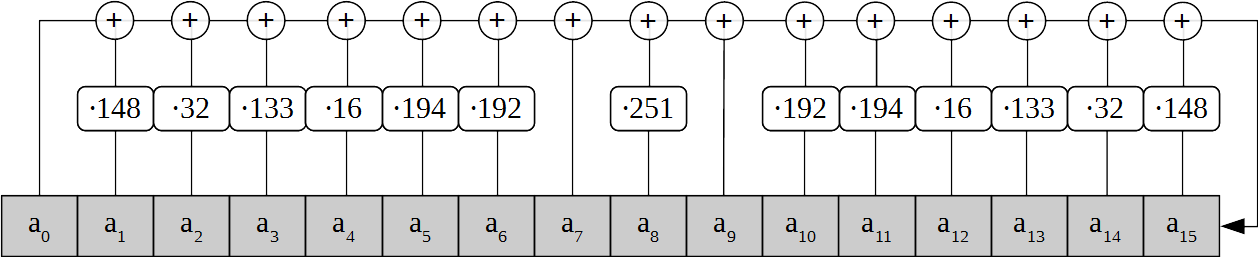
\includegraphics[scale=0.5]{image2.png}}
\label{fig:image}
\end{figure}

    \hfill \break
Раундовое преобразование можно изобразить следующим образом:


\begin{figure}[h]
\center{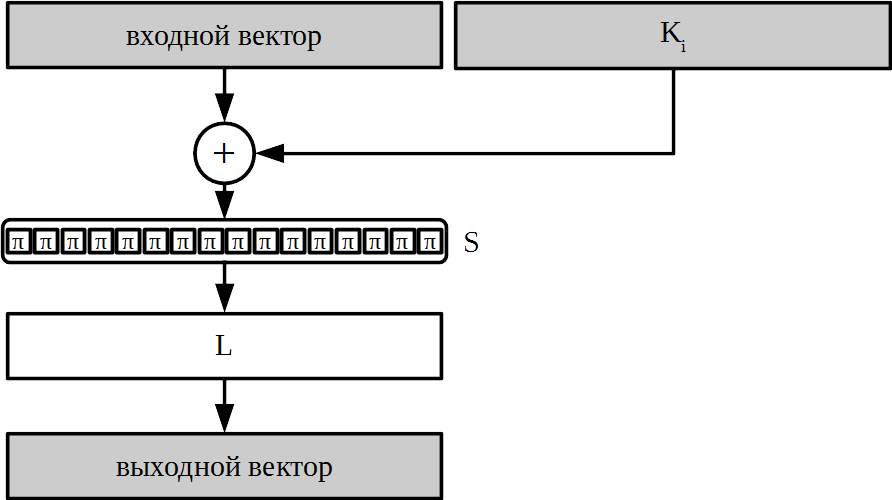
\includegraphics[scale=0.5]{image3.png}}
\label{fig:image}
\end{figure}

  \subsection{Выработка раундовых ключей}

Рассмотрим теперь процедуру генерации раундовых ключей из мастер-ключа. Первые два получаются разбиением мастер-ключа пополам. Далее для выработки очередной пары раундовых ключей используется 8 итераций сети Фейстеля, где, в свою очередь, в качестве раундовых ключей используется счетчиковая последовательность, прошедшая через линейное преобразование алгоритма:

$F[k]: V_{128} \times V_{128} \rightarrow F[k](a_{1}, a_{0}) = (LSX[k](a_{0}, a_{1}))$
    \hfill \break
    
Раунд ключевой развертки можно представить следующим образом:

\begin{figure}[h]
\center{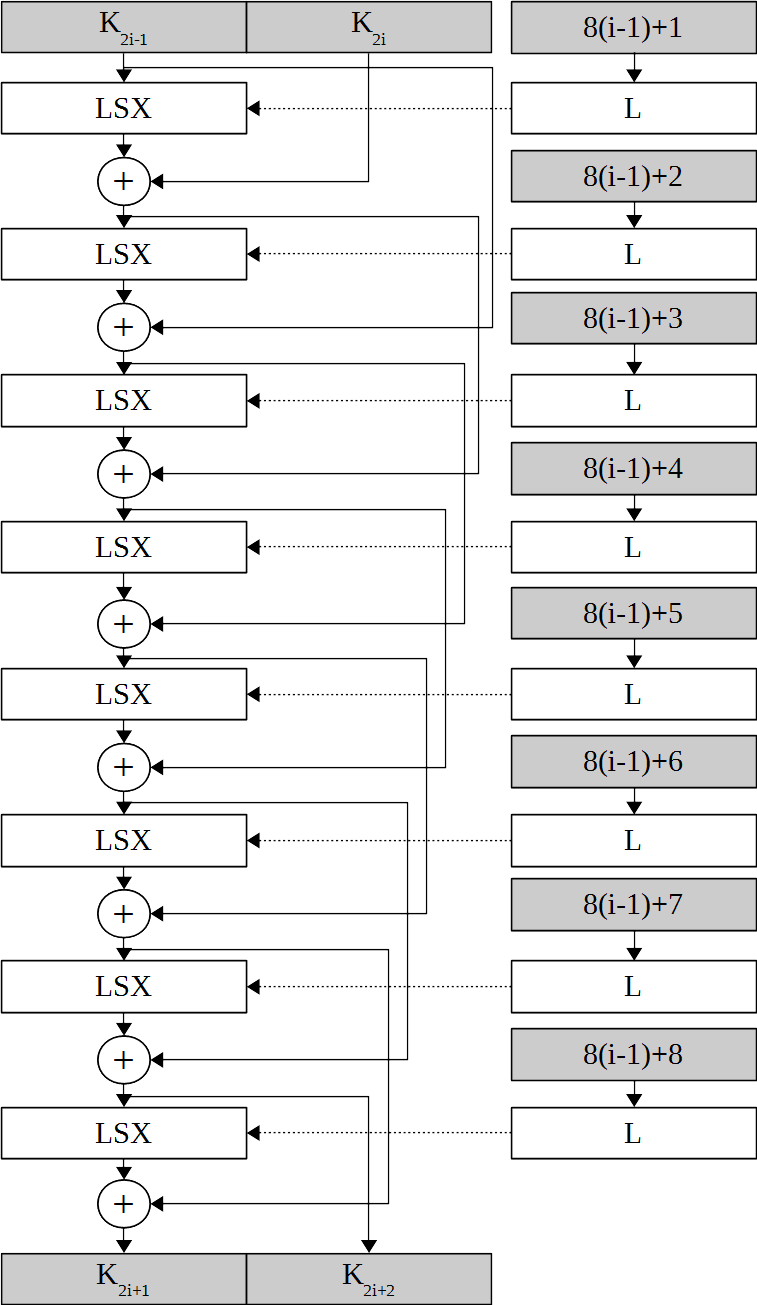
\includegraphics[scale=0.4]{image4.png}}
\label{fig:image}
\end{figure}

А всю процедуру выработки раундовых ключей так:

\begin{figure}[h]
\center{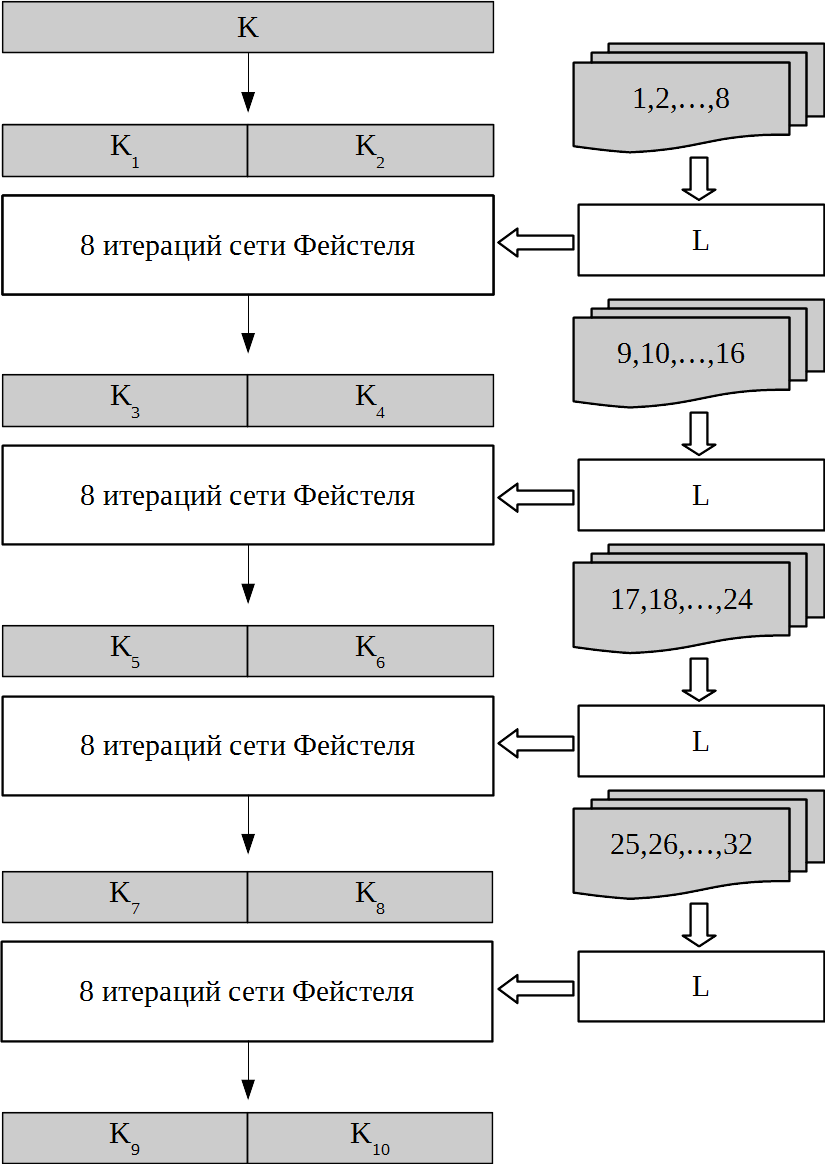
\includegraphics[scale=0.3]{image5.png}}
\label{fig:image}
\end{figure}



\subsection{Шифрование и расшифрование}

В результате, шифрование одного 128-битного входного блока описывается следующим уравнением:

$E_{K_{1}...,K{10}}(a) = X[K_{10}]LSX[K_{2}]LSX[K_{1}](a),$

А в виде блок-схемы может быть представлено так:

\begin{figure}[h]
\center{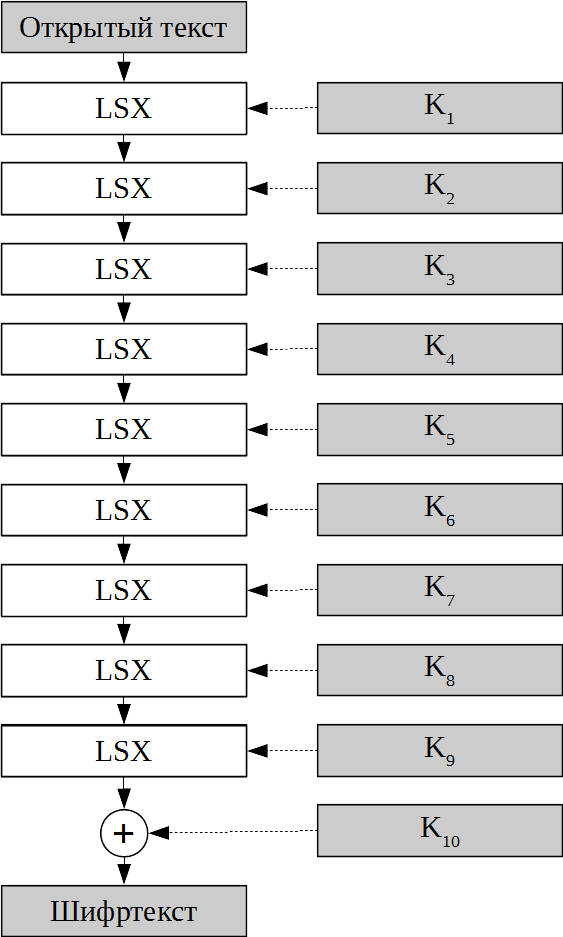
\includegraphics[scale=0.5]{image6.png}}
\label{fig:image}
\end{figure}

Расшифрование реализуется обращением базовых преобразований и применением их в обратном порядке:

$D_{K_{1}...,K{10}}(a) = X[K_{1}]S^{-1}L^{-1}X[K_{2}]...S^{-1}L^{-1}X[K_{9}]S^{-1}L^{-1}X[K_{10}](a)$

\chapter{Реализация и использование программы Hash Streebog}
\subsection{Возможности Hash Streebog}

\textbf{Hash Streebog} представляет из себя приложение для Windows,  для проверки целостности и подлинности файлов посредством вычисления контрольной суммы.

\textbf{Hash Streebog} использует алгоритм хеширования, \textbf{ГОСТ Р 34.11-2012 - Стрибог} с функцией длиной выходного значения в \textbf{256 бит} и функцию с дилной входного значения в \textbf{512 бит}. Обе эти функции имеют одинаковую структуру и отличаются друг от друга только начальным внутренним состоянием. Выходным данными для обеих функций является блок данных длиной \textbf{512 бит}. В случае, если длина сообщения больше \textbf{512 бит}, то происходит разбиение сообщения на блоки. В случае же, если длина меньше \textbf{512 бит}, то производится дополнение сообщения. 

\subsection{Использование Hash Streebog}

Основное окно приложения \textbf{Hash Streebog} интуитивно понятно, для добавления файлов или же целых папок требуется перейти во вкладку \textbf{Add} - которая находится в \textbf{menuStrip}

\begin{figure}[h]
\center{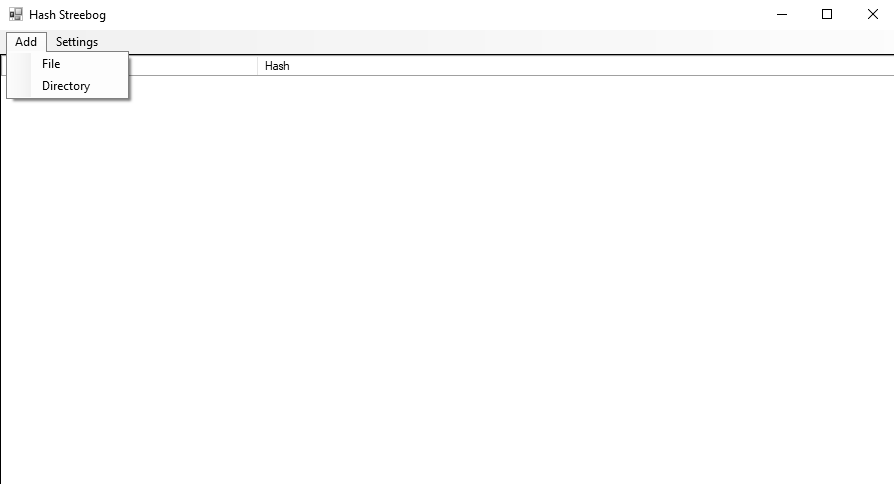
\includegraphics[scale=0.3]{Streebog-1.png}}
\caption{Основное окно взаимодействия и добавления файлов для получения хэш-функции}
\label{fig:image}
\end{figure}

Для изменения входного значения функции, требуется перейти во вкладку \textbf{Settings} - которая находится в \textbf{menuStrip}, в \textbf{Hash code size}, можно выбрать размер входной функции \textbf{256 бит}, которая стоит по стандарту, или же \textbf{512 бит}

\begin{figure}[h]
\center{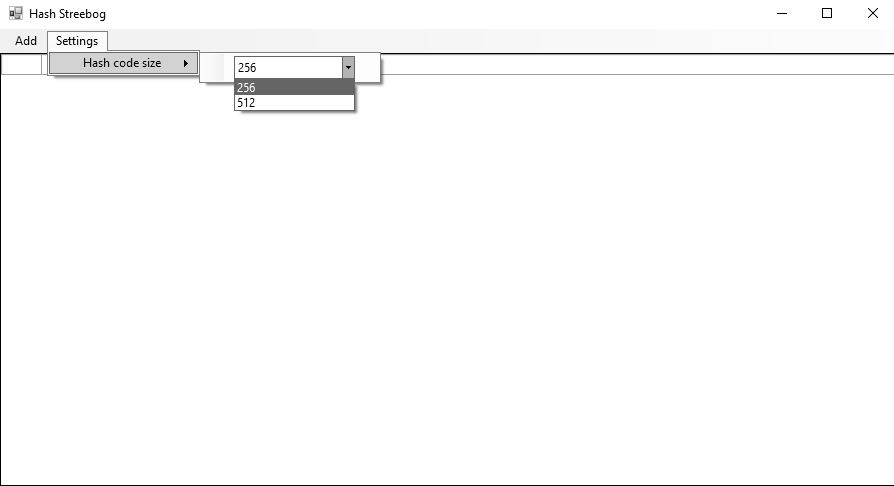
\includegraphics[scale=0.3]{Streebog-2.png}}
\caption{Окно выбора размера входной функции}
\label{fig:image}
\end{figure}

\subsection{Литература и ссылки на скачивания}

Статистическое тестирование российского стандарта функции хэширования ГОСТ 34.11-2012:

https://cyberleninka.ru/article/n/statisticheskoe-testirovanie-rossiyskogo-standarta-funktsii-heshirovaniya-gost-34-11-2012-stribog
 \hfill \break
 
Дифференциальный анализ шифра Кузнечик:

 https://cyberleninka.ru/article/n/differentsialnyy-analiz-shifra-kuznechik
  \hfill \break

 А.П. Алферов, А. Ю. Зубов, А. С. Кузьмин,  А.В. Черемушкин Основы криптографии:
 
  https://studfile.net/preview/6311470/
  \hfill \break
  
Контрольная сумма:

https://studfile.net/preview/6211065/page:7/
 \hfill \break
 
 Некоторые методы анализа 
функций хэширования и их применение к алгоритму ГОСТ 
Р 34.11-94:

http://www.mathnet.ru/links/aef9a4396008a1c6d22235edbaa62714/mvk68.pdf
 \hfill \break
 
 Hash Streebog: 
 
https://github.com/danrom11/HashStreebog

\end{document}  